\documentclass[12pt, twoside]{article}
\usepackage[francais]{babel}
\usepackage[T1]{fontenc}
\usepackage[latin1]{inputenc}
\usepackage[left=7mm, right=7mm, top=7mm, bottom=7mm]{geometry}
\usepackage{float}
\usepackage{graphicx}
\usepackage{array}
\usepackage{multirow}
\usepackage{amsmath,amssymb,mathrsfs}
\usepackage{textcomp}
\pagestyle{empty}
\usepackage{soul}

\begin{document} 


\begin{center}
{\fbox{$4^{e}4$ \qquad \qquad \textbf{\Large{Devoir surveill� 6 (sujet 1)}}
\qquad \qquad 09/03/2012}}
\end{center}

\bigskip

\bigskip


\ul{\textbf{Exercice 1}}: (\textit{2 points})

\begin{enumerate}
  \item Le nombre -4 est-il solution de l'�quation 7y-6=15-3y? Justifier votre
  r�ponse.
  \item Le nombre 5 est-il solution de l'�quation 4t-21=-1? Justifier votre
  r�ponse. 
\end{enumerate}

\bigskip


\bigskip

\ul{\textbf{Exercice 2}}: (\textit{3 points})

\enskip

R�soudre les �quations suivantes: \quad \quad  u-7=-10 \quad \qquad \qquad
2z=-21 \quad \qquad \qquad -3a+5=23


\bigskip

\bigskip


\ul{\textbf{Exercice 3}}: (\textit{2 points})



\begin{tabular}{cc}
\begin{minipage}{14cm}
Calculer la longueur DF. On donnera une valeur arrondie au millim�tre.
\end{minipage}
&
\begin{minipage}{5cm}
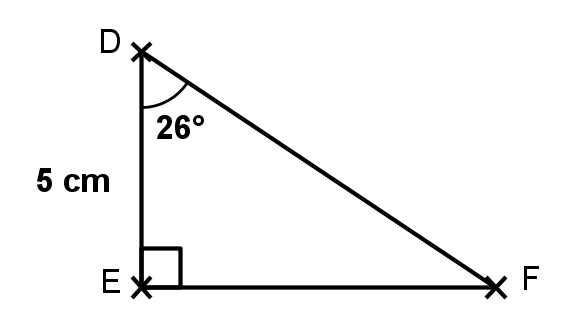
\includegraphics[width=4cm]{images/ex3-sujet1.png}
\end{minipage}
\end{tabular}



\bigskip

\bigskip

\ul{\textbf{Exercice 4}}: (\textit{4 points})


\begin{tabular}{cc}
\begin{minipage}{14cm}
\begin{enumerate}
  \item Calculer la longueur GH. On donnera une valeur arrondie au centim�tre.
  \item Calculer la longueur HI. On donnera une valeur arrondie au centim�tre.
\end{enumerate}
\end{minipage}
&
\begin{minipage}{5cm}
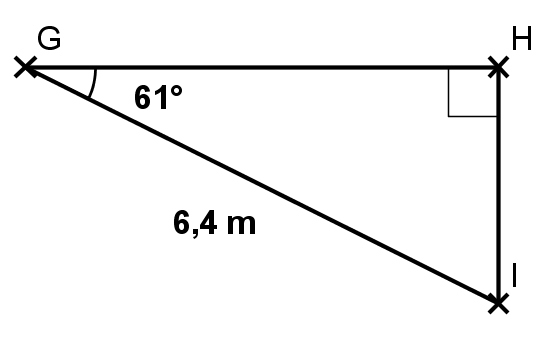
\includegraphics[width=4cm]{images/ex4-sujet1.png}
\end{minipage}
\end{tabular}


\bigskip

\bigskip

\ul{\textbf{Exercice 5}}: (\textit{3 points})

\enskip

KLM est un triangle rectangle en K v�rifiant KL=6km et LM=11km.
\begin{enumerate}
  \item Calculer la mesure de l'angle $\widehat{KLM}$. On donnera une valeur
  arrondie au degr�.
  \item En d�duire une mesure de l' angle $\widehat{KML}$. 
\end{enumerate}


\bigskip

\bigskip


\ul{\textbf{Exercice 6}}: (\textit{6 points + 1 point BONUS})

\enskip

\begin{tabular}{cc}
\begin{minipage}{12cm}

 Sur la figure ci-contre, les droites (MN) et (BC) sont parall�les et AB=10cm.
 
 \begin{enumerate}
   \item Montrer que AC=8cm. Justifier votre r�ponse.
   \item Calculer BC. Justifier votre r�ponse.
   
   \textbf{Pour la suite des questions, on admettra que BC=6cm.}
   
   
   \item Montrer que le triangle ABC est rectangle.
   \item Calculer la mesure de l'angle $\widehat{ABC}$. Arrondir au degr�.
   \item BONUS: En d�duire une mesure de l'angle $\widehat{AMN}$.
 \end{enumerate}
\end{minipage}
&
\begin{minipage}{6cm}
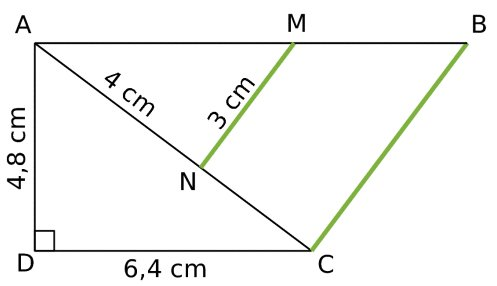
\includegraphics[width=6cm]{images/ex4.jpg}
\end{minipage}
\end{tabular}


\pagebreak


\begin{center}
{\fbox{$4^{e}4$ \qquad \qquad \textbf{\Large{Devoir surveill� 6 (sujet 2)}}
\qquad \qquad 09/03/2012}}
\end{center}

\bigskip

\bigskip


\ul{\textbf{Exercice 1}}: (\textit{2 points})

\begin{enumerate}
  \item Le nombre -3 est-il solution de l'�quation 8b-4=12-7b? Justifier votre
  r�ponse.
  \item Le nombre 6 est-il solution de l'�quation 5y-31=-1? Justifier votre
  r�ponse. 
\end{enumerate}

\bigskip


\bigskip

\ul{\textbf{Exercice 2}}: (\textit{3 points})

\enskip

R�soudre les �quations suivantes: \quad \quad  t-8=-12 \quad \qquad \qquad
4u=-10 \quad \qquad \qquad -2a+7=21


\bigskip

\bigskip


\ul{\textbf{Exercice 3}}: (\textit{2 points})



\begin{tabular}{cc}
\begin{minipage}{14cm}
Calculer la longueur NP. On donnera une valeur arrondie au millim�tre.
\end{minipage}
&
\begin{minipage}{5cm}
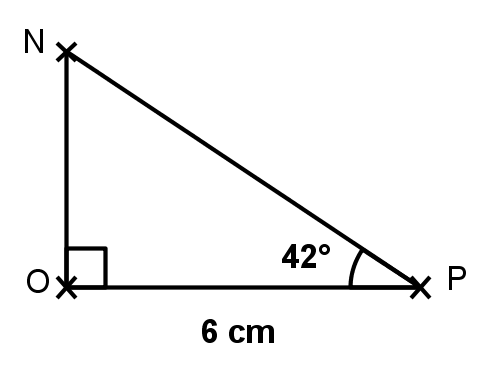
\includegraphics[width=4cm]{images/ex3-sujet2.png}
\end{minipage}
\end{tabular}



\bigskip

\bigskip

\ul{\textbf{Exercice 4}}: (\textit{4 points})


\begin{tabular}{cc}
\begin{minipage}{14cm}
\begin{enumerate}
  \item Calculer la longueur ST. On donnera une valeur arrondie au centim�tre.
  \item Calculer la longueur RS. On donnera une valeur arrondie au centim�tre.
\end{enumerate}
\end{minipage}
&
\begin{minipage}{5cm}
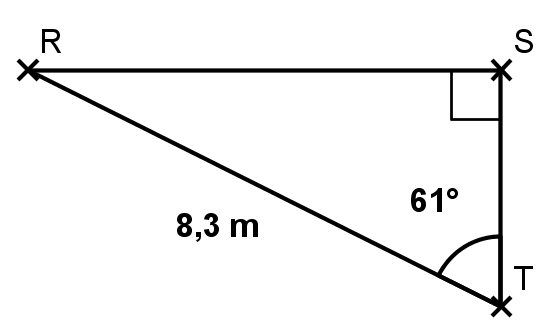
\includegraphics[width=4cm]{images/ex4-sujet2.png}
\end{minipage}
\end{tabular}


\bigskip

\bigskip

\ul{\textbf{Exercice 5}}: (\textit{3 points})

\enskip 

KLM est un triangle rectangle en K v�rifiant KL=6km et LM=11km.
\begin{enumerate}
  \item Calculer la mesure de l'angle $\widehat{KLM}$. On donnera une valeur
  arrondie au degr�.
  \item En d�duire une mesure de l' angle $\widehat{KML}$. 
\end{enumerate}


\bigskip

\bigskip


\ul{\textbf{Exercice 6}}: (\textit{6 points + 1 point BONUS})

\enskip

\begin{tabular}{cc}
\begin{minipage}{12cm}

 Sur la figure ci-contre, les droites (MN) et (BC) sont parall�les et AB=10cm.
 
 \begin{enumerate}
   \item Montrer que AC=8cm. Justifier votre r�ponse.
   \item Calculer BC. Justifier votre r�ponse.
   
   \textbf{Pour la suite des questions, on admettra que BC=6cm.}
   
   
   \item Montrer que le triangle ABC est rectangle.
   \item Calculer la mesure de l'angle $\widehat{ABC}$. Arrondir au degr�.
   \item BONUS: En d�duire une mesure de l'angle $\widehat{AMN}$.
 \end{enumerate}
\end{minipage}
&
\begin{minipage}{6cm}
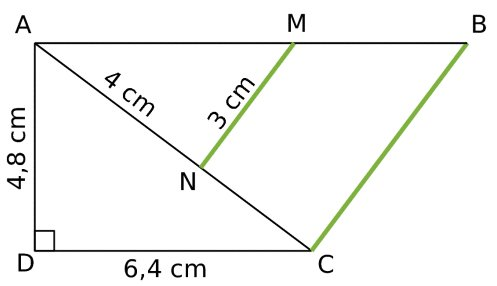
\includegraphics[width=6cm]{images/ex4.jpg}
\end{minipage}
\end{tabular}
\end{document}
